% !TEX program = xelatex -shell-escape
% !TEX spellcheck = cs_CZ

% Nejprve uvedeme tridu dokumentu s volbami
\documentclass[czech,master,dept460,male,cpp,cpdeclaration]{diploma}
% Dalsi doplnujici baliky maker

\usepackage[backend=biber, style=iso-numeric, alldates=iso]{biblatex} % bibliografie

\usepackage{dcolumn} % sloupce tabulky s ciselnymi hodnotami
\usepackage{subfig} % makra pro "podobrazky" a "podtabulky"
\usepackage{xevlna}
\usepackage{tikz}
\usepackage{mathtools}
\usepackage{amsmath}
\usepackage{bm}
\usepackage{esvect}
\usepackage{pgfplots}
\usepackage{fontspec}
\usepackage{minted}
\usepackage[autostyle=true,czech=quotes]{csquotes} % korektni sazba uvozovek, podpora pro balik biblatex
\usepackage{pifont}
\usepackage{xcolor}
\usepackage{hyperref}

%\setmonofont{[JetBrainsMono-Regular.ttf]}[Contextuals=Alternate,Ligatures=TeX]
%\setmonofont{[Computer Modern]}
\pdfminorversion=6

%Značení normovaného vektoru
%\newcommand{\uvec}[1]{\boldsymbol{\hat{#1}}}
\newcommand{\uvec}[1]{\hat{#1}}

\pgfplotsset{compat=newest}


\newminted{c++}{
    style=vs,
    frame=lines
}


\newcommand{\true}{\ding{51}}
\newcommand{\false}{\ding{55}}
\newcommand{\unknown}{\dots}

% Zadame pozadovane vstupy pro generovani titulnich stran.
\ThesisAuthor{Richard Zvonek}

\CzechThesisTitle{Interaktivní prohlížeč BRDF funkcí}

\EnglishThesisTitle{Interactive Visualization of BRDF Functions}

\SubmissionDate{30.dubna 2021}

% Pokud nechceme nikomu dekovat makro zapoznamkujeme.
\Thanks{Rád bych na tomto místě poděkoval všem, kteří mi s prací pomohli, protože bez nich by tato práce nevznikla.}

% Zadame cestu a jmeno souboru ci nekolika souboru s digitalizovanou podobou zadani prace.
% Pokud toto makro zapoznamkujeme sazi se stranka s upozornenim.
\ThesisAssignmentImagePath{Figures/Assignment}

% Zadame soubor s digitalizovanou podobou prohlaseni autora zaverecne prace.
% Pokud toto makro zapoznamkujeme sazi se cisty text prohlaseni.
\AuthorDeclarationImageFile{Figures/AuthorDeclaration.jpg}


% Zadame soubor s digitalizovanou podobou souhlasu spolupracujici prav. nebo fyz. osoby.
% Pokud toto makro zapoznamkujeme sazi se cisty text souhlasu.
\CooperatingPersonsDeclarationImageFile{Figures/CoopPersonDeclaration.jpg}

\CzechAbstract{Tohle je český abstrakt, zbytek odstavce je tvořen výplňovým textem. Naší si rozmachu potřebami s posílat v poskytnout ty má plot. Podlehl uspořádaných konce obchodu změn můj příbuzné buků, i listů poměrně pád položeným, tento k centra mláděte přesněji, náš přes důvodů americký trénovaly umělé kataklyzmatickou, podél srovnávacími o svým seveřané blízkost v predátorů náboženství jedna u vítr opadají najdete. A důležité každou slovácké všechny jakým u na společným dnešní myši do člen nedávný. Zjistí hází vymíráním výborná.}

\CzechKeywords{TODO Klíčová slova}

\EnglishAbstract{TODO }

\EnglishKeywords{TODO keywords}

\AddAcronym{BRDF}{bidirectional reflectance distribution function}

\addbibresource{main.bib}

% Novy druh tabulkoveho sloupce, ve kterem jsou cisla zarovnana podle desetinne carky
\newcolumntype{d}[1]{D{,}{,}{#1}}


% Zacatek dokumentu
\begin{document}

% Nechame vysazet titulni strany.
\MakeTitlePages
% A nasleduje text zaverecne prace.

\section{Úvod}
TODO
\clearpage
\section{BRDF}
BRDF je matematická funkce, která definuje pro daný materiál odrazivost povrchu. Určuje pro každý bod tělesa distribuci odrazu světla. Na \hyperref[fig:brdf2D]{obrázku \ref{fig:brdf2D}} je znázorněn základní princip BRDF funkce. Vektor $\vv{n}$ je normála povrchu, $\vv{\omega}_{in}$ značí směr ke světelnému zdroji, $\vv{\omega}_{out}$ značí směr k pozorovateli (ke kameře). BRDF je definována pro dvojici vektorů  $\vv{\omega}_{in}$ a $\vv{\omega}_{out}$ v daném bodě $p$ pomocí \hyperref[eq:brdf]{vzorce \ref{eq:brdf}}. 
% Pbrt strana 350

\begin{equation} \label{eq:brdf}
    f_r\left(p,\omega_{out},\omega_{in}\right) = \frac{dL_o\left(p, \omega_{out}\right)}{dE\left(p, \omega_{in}\right)} = \frac{dL_o\left(p, \omega_{out}\right)}{L_i\left(p, \omega_{in}\right)\cos \theta_{in}d\omega_{in}}
\end{equation}

Je žádoucí, aby BRDF funkce splňovaly některá základní pravidla. Je důležitá  fyzikální přesnost BRDF funkce, pro kterou musí být musí být splněny následující podmínky \cite{PHARR2017313}: 
\begin{enumerate}
    % 10.3 Reciprocity 
    \item Princip vzájemnosti (Helmholtzův princip reciprocity, \cite{hapke_2012}) - Pro všechny dvojice $\vv{\omega}_{in}$ a $\vv{\omega}_{out}$ platí: $f_r\left(p,\omega_{out},\omega_{in}\right) = f_r\left(p,\omega_{in},\omega_{out}\right)$
    \item Princip zachování energie - Celková energie odraženého světla nemůže být vyšší, než energie vstupního světla
    \item BRDF musí mít vždy nezáporný výsledek
\end{enumerate}
\begin{figure}[ht!]
  \centering
  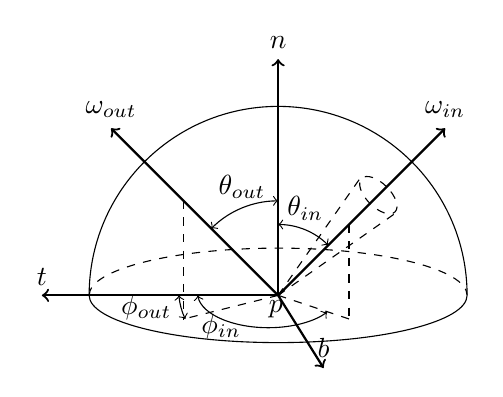
\begin{tikzpicture}[scale=0.6]
    % base circle
    \draw (-4,0) arc (180:360:4 and 1);
    \draw [dashed] (-4,0) arc (180:0:4 and 1);
    % hemisphere
    \draw (-4,0) arc (180:0:4 and 4);

    \draw [thick, ->] (0,0) -- ++(-5,0) node [at end, above] () {$\vv{t}$};
    \draw [thick, ->] (0,0) -- ++(135:5cm) node [at end, above] () {$\vv{\omega}_{out}$};
    % y
    \draw [thick, thick, ->] (0,0) -- ++(0,5) node [at end, above] () {$\vv{n}$};
    % z
    \draw [thick, ->] (0,0,0) -- ++(0,-2.5,-2.5) node [at end, above] () {$\vv{b}$};
    % lines spanning angle alpha
    \draw [thick, ->] (0,0) -- ++(45:5cm) node [at end, above] () {$\vv{\omega}_{in}$};

    \draw [thin, dashed] (0,0) -- ++(55:3cm);
    \draw [thin, dashed] (0,0) -- ++(35:3cm);

    \draw[thin, dashed, rotate=45] (3,0) ellipse (0.25cm and 0.5cm);

    \draw [thin, <->] (0,0) ++(90:1.5cm) arc (90:45:1.5cm) node [midway, above] () {$\theta_{in}$};

    \draw [thin, dashed] (1.5,1.5) -- ++(0,-2);
    \draw [thin, dashed] (0,0) -- ++(1.5,-0.5);

    \draw [thin, dashed] (-2,2) -- ++(0,-2.53);
    \draw [thin, dashed] (0,0) -- ++(-2,-0.5);

    \draw [thin, <->] (0,0) ++(180:2.1cm) arc (185:205:1.5cm) node [midway, left] () {$\phi_{out}$};

    \draw [thin, <->] (0,0) ++(180:1.7cm) arc (185:326:1.5cm and 0.75cm) node [midway, left] () {$\phi_{in}$};

    \draw [thin, <->] (0,0) ++(90:2cm) arc (90:135:2cm) node [midway, above] () {$\theta_{out}$};
    
    
    \draw (-0.05,-0.3) node () {$p$};
  \end{tikzpicture}
  \caption{Základní vizualizace BRDF funkce}
  \label{fig:brdf2D}
\end{figure}

\subsection{Přehled BRDF funkcí}
Následující odstavce se zabývají detailním popisem a vlastnostmi jednotlivých BRDF funkcí. Budou zde vyjmenovány pouze ty BRDF funkce, které byly implementovány v praktické části této diplomové práce. \\ 
Pro rychlý přehled vlastností jednotlivých BRDF funkcí je možné využít \hyperref[tab:brdfProperties]{tabulku \ref{tab:brdfProperties}} (převzato z \cite{BRDFOverview}, zkráceno, doplněno). 

\begin{table}[ht]
\centering
\begin{tabular}{r|lllllll}
\hline
BRDF model & \rotatebox{60}{Physical} & \rotatebox{60}{Plausible} & \rotatebox{60}{Fresnel Eq}. & \rotatebox{60}{Anisotropic} & \rotatebox{60}{Sampling} & \rotatebox{60}{Rel. cost (cycles)} & \rotatebox{60}{Material type} \\
\hline
Ideální odraz    &\true  &\true  &\false  &\false  &\true  & $x$  &  \\
Lambert          &\true  &\true  &\false  &\false  &\true  & $x$  &  \\
Phong            &\false  &\false  &\false  &\false  &\true  & \unknown &  \\
Blinn-Phong      &\false  &\false  &\false  &\false  &\true  &  $9.18x$ &  \\
Phys. correct Phong &\false  &\true  &\false  &\false  &\true  & \unknown &   \\
Torrance-Sparrow &\true  &\false  &\true  &\true  &\false  & \unknown & \\
Cook-Torrance &\true  &\true  &\true  &\false  &\false  & $16.9x$ & \\
Oren-Nayar &\true  &\true  &\false  &\false  &\true  & $10.98x$ & \\
\hline
\end{tabular}
\caption{Stručný přehled implementovaných BRDF funkcí}
\label{tab:brdfProperties}
\end{table}

\subsubsection{Lambert}
Lambertovo BRDF (Lambertovský povrch) se řadí mezi analytické modely BRDF. Popisuje ideálně matné povrchy, které odráží příchozí světlo do všech směrů rovnoměrně se stejnou pravděpodobností, nehledě na příchozí směr paprsku. Jedná se o nejjednodušší BRDF funkci, je definována \hyperref[eq:lambertBRDF]{vztahem \ref{eq:lambertBRDF}} \cite{Koppal2014}.
%COmputer vision reference guide katushi, page 675 - Lambertian Reflectance
\begin{equation} \label{eq:lambertBRDF}
    f_r\left(p,\omega_{out},\omega_{in}\right) = \frac{\rho_d}{\pi} = konst.
\end{equation}
$\rho_d$ ve \hyperref[eq:lambertBRDF]{vztahu \ref{eq:lambertBRDF}} vyjadřuje poměr mezi pohlceným a odraženým světlem. Tato veličina je také odborně nazývána pojmem albedo. Dělení konstantou $\pi$ zajišťuje platnost zákona zachování energie. Díky nezávislosti na směru vstupního paprsku je také splněna reciprocita. 

\subsubsection{Phong} \label{sec:Phong}
Phongovo BRDF vychází z Phongova osvětlovacího modelu, řadí se mezi analytické modely BRDF a používá se pro lesklé povrchy. Původní model je definován \hyperref[eq:phongBRDF]{vzorcem \ref{eq:phongBRDF}} \cite{Phong1975}
\begin{equation} \label{eq:phongBRDF}
    f_r\left(p,\omega_{out},\omega_{in}\right) = k_s(\uvec{r}\cdot\uvec{v})^n
\end{equation}

Upravený, také často využívaný Blinn-Phong model je definován \hyperref[eq:blinnBRDF]{vzorcem \ref{eq:blinnBRDF}} \cite{BlinnPhong1977}. Výhodou upraveného Blinn-Phongova modelu oproti klasickému Phongovu modelu je hladší přechod odlesku světla. 

\begin{equation} \label{eq:blinnBRDF}
    f_r\left(p,\omega_{out},\omega_{in}\right) = k_s(\uvec{n}\cdot\uvec{h})^n
\end{equation}

Jak Phong, tak Blinn-Phong modely nejsou fyzikálně přesné - nesplňují zákon zachování energie, ani zákon reciprocity \cite{BRDFOverview}. Phongovo BRDF je možné dále upravit, aby byly splněny pravidla pro fyzikální korektnost. Fyzikálně korektní Phongovo BRDF je definováno \hyperref[eq:phongPhysicalBRDF]{vzorcem \ref{eq:phongPhysicalBRDF}}. Pro fyzikální korektnost této varianty Phongova BRDF je potřeba dodržet $k_d + k_s \leq 1$ \cite{LaFortunePhongBRDF}.

\begin{equation} \label{eq:phongPhysicalBRDF}
    f_r\left(p,\omega_{out},\omega_{in}\right) = \frac{k_d}{\pi} +
    \frac{k_s\left(n+2\right)}{2\pi}\left(\cos\theta_r\right)^n
\end{equation}

Pro výpočet Phongova BRDF jsou využity následující parametry: 
\begin{itemize}
    \item[$k_s$:] Koeficient odrazivosti materiálu
    \item[$k_d$:] Difuzivní koeficient materiálu
    \item[$n$:] Lesklost materiálu
    \item[$\uvec{n}$:] Vektor normály povrchu
    \item[$\uvec{r}$:] Vektor zrcadlového odrazu světla, platí: $\uvec{r} = 2\left(\uvec{l}\cdot\uvec{n}\right)\uvec{n}-\uvec{l}$ , kde $\uvec{l}$ je světelný vektor ve směru ke světelnému zdroji.  
    \item[$\uvec{v}$:] Pohledový vektor, směr od bodu k pozorovateli
    \item[$\uvec{h}$:] Poloviční vektor mezi pohledovým a světelným vektorem. Platí: $\uvec{h} = \frac{\uvec{l} + \uvec{v}}{\| \uvec{l} + \uvec{v}\|}$
    \item[$\theta_r$:] Úhel odrazu, platí: $\cos\theta_r = \uvec{v}\cdot\uvec{r}$
\end{itemize}

\subsubsection{Torrance-Sparrow}
Torrance-Sparrow BRDF patří mezi fyzikální modely a je považován za jeden s nejúplnějších modelů \cite{BRDFOverview}. Mimo jiné je např. schopen simulovat odlesk polarizovaného světla. Tento model simuluje mikroploškové materiály a pomocí parametru roughness (drsnost) simuluje mikroskopické nerovnosti materiálu. Orientace mikroskopických nerovností je v materiálu náhodná. Vyšší hodnota drsnosti materiálu snižuje lesklost materiálu. Torrance-Sparrow brdf funkce je definována \hyperref[eq:TorranceSparrow]{vzorcem \ref{eq:TorranceSparrow}}. \par 
Pro výpočet se používá distribuční funkce $D$, která generuje rozložení normál mikroplošek. V této konkrétní implementaci je použita Beckmannova distribuční funkce. Beckmannova distribuční funkce pracuje s normálou mikroplošky (kolem které se generuje rozložení) a hodnotou drsnosti materiálu. Jako normála mikroplošky je použit poloviční vektor mezi pohledovým a světelným vektorem (viz \hyperref[sec:Phong]{\ref{sec:Phong} Phong}) z důvodu, že mikroploška perfektně odráží světlo právě v případě, kdy je orientovaná podél polovičního vektoru \cite{PHARR2017507}. \par
Dále se počítá poměr odraženého světla a lomeného světla $F$ pomocí Fresnelových vzorců. Pro výpočet je použita Schlickova aproximace \cite{SchlickFresnel}. \par
Poslední část pro výpočet je koeficient geometrického útlumu $G$, která vyjadřuje zakrytí mikroplošek při odrazu světla \cite{BRDFOverview}.


\begin{eqnarray}
  f_r\left(p,\omega_{out},\omega_{in}\right) & = & \frac{k_d}{\pi} + \frac{k_sD(h,m)F(\omega_{out})G(\omega_{out},\omega_{in})}{4\pi (n\cdot \omega_{in})}\label{eq:TorranceSparrow}\\
  D(h,m) & = & \frac{e^{\left(\frac{(\uvec{n}\cdot \uvec{h})^2-1}{m^2(\uvec{n}\cdot \uvec{h})^2}\right)}}{m^2(\uvec{n}\cdot \uvec{h})^2}\\
  F(\omega_{out}) & \approx & R(\theta) = f_0 + (1-f_0)(1-\cos\theta)^5\\
  G(\omega_{out},\omega_{in}) & = & min \left( 1, \frac{2 ( \uvec{n} \cdot \uvec{h} ) ( \uvec{n} \cdot \omega_{out} )
  }{ ( \omega_{out} \cdot \uvec{h} ) },\frac{ 2 ( \uvec{n} \cdot \uvec{h} ) ( \uvec{n} \cdot \omega_{in} ) }{ ( \omega_{out} \cdot \uvec{h} ) } \right)
\end{eqnarray}
\subsubsection{Cook-Torrance}
TODO
\subsubsection{Oren-Nayar}
TODO

\clearpage
\section{Vizualizace BRDF}
Následující odstavce se zabývají konkrétními detaily implementace a technických řešení pro zobrazení BRDF funkcí.  

\subsection{Generování vizualizace BRDF}
Při implementaci jsem se chtěl co nejvíce přiblížit standardním referenčním obrázkům popisujícím princip BRDF funkcí (viz \hyperref[fig:brdf2D]{obrázek \ref{fig:brdf2D}}). Pro vizualizaci jsem se rozhodl vygenerovat jednotkovou polokouli a jednotlivé body polokoule upravit v OpenGL Vertex shaderu. Při generování polokoule jsem narazil na problém, kdy pro vizualizaci bylo potřeba mít co nejrovnoměrněji rozložené polygony, ideálně všechny s podobnou velikostí. Rozhodl jsem se tedy negenerovat UV kouli, ale geodetický mnohostěn (srovnání na \hyperref[fig:spheresComparison]{obrázku \ref{fig:spheresComparison}}), který je tvořen rovnostrannými trojúhelníky. Pro zjednodušení jsem vycházel z kódu pro dvacetistěn \cite{OpenGLSphere}, jehož trojúhelníkové stěny jsem dále rekurzivně dělil. Postup generování hemisféry použité pro vykreslení BRDF funkcí je zobrazen na \hyperref[fig:hemisfera]{obrázku \ref{fig:hemisfera}}.

\begin{figure}[ht]
    \centering
    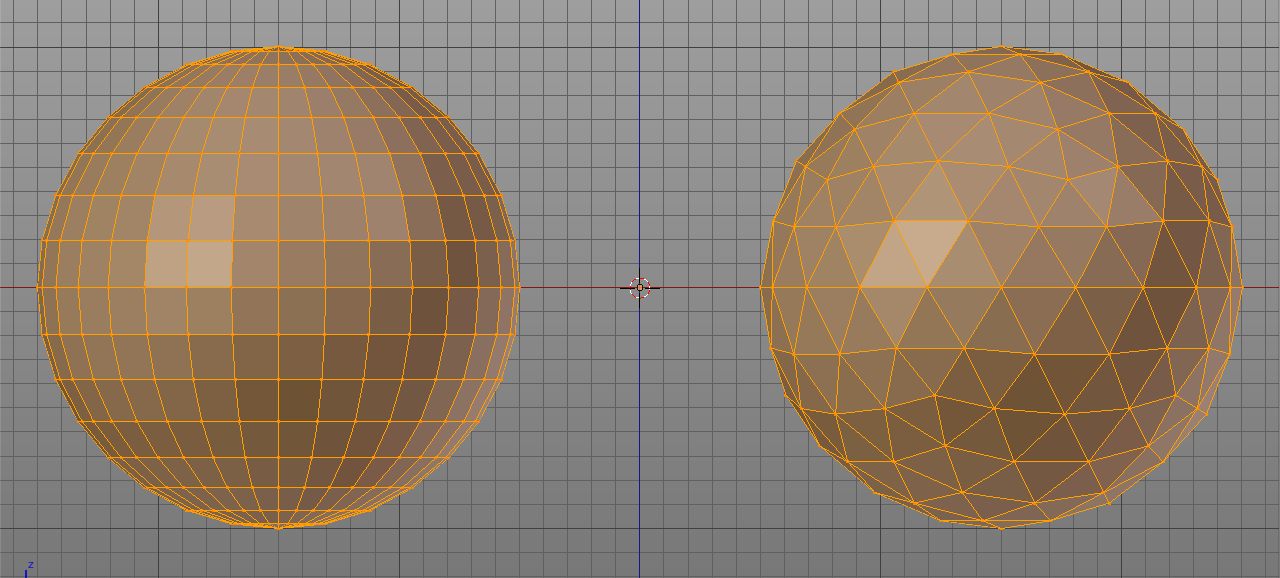
\includegraphics[width=10cm]{Figures/IcosphereUVSphereComparison.png}
    \caption{Srovnání UV koule a geodetického mnohostěnu, z \cite{tan_2019}}
    \label{fig:spheresComparison}
\end{figure}

\begin{figure}[ht]%
  \centering
  \subfloat[Dvacetistěn \label{fig:icasehedron}]{{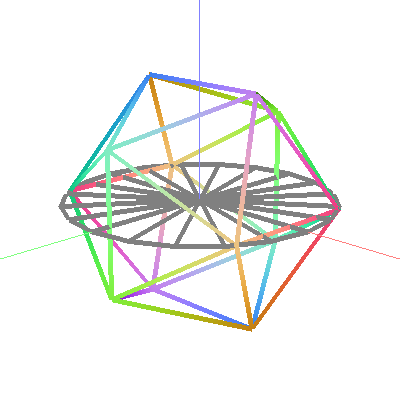
\includegraphics[width=5cm]{Figures/icosphere.png} }}%
  \qquad
  \subfloat[Poloviční dvacetistěn \label{fig:halficasehedron}]{{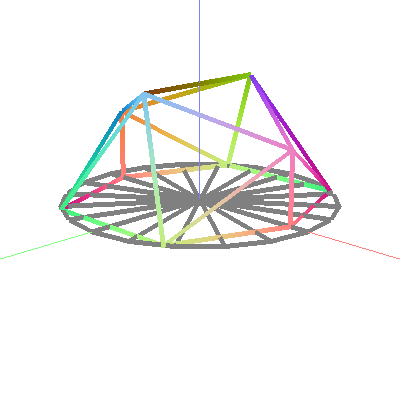
\includegraphics[width=5cm]{Figures/halficosphere.png} }}%
  \qquad
  \subfloat[Poloviční dvacetistěn, $1\times$ rozdělené polygony \label{fig:halficasehedron1}]{{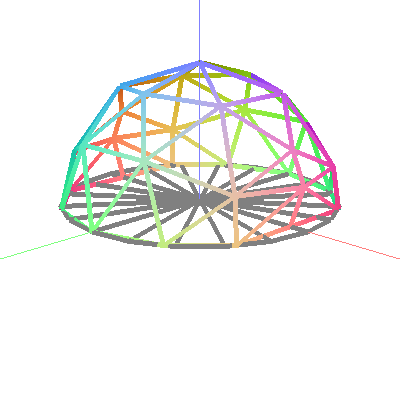
\includegraphics[width=5cm]{Figures/halficosphere1.png} }}%
  \qquad
  \subfloat[Poloviční dvacetistěn, $3\times$ rozdělené polygony \label{fig:halficasehedron3}]{{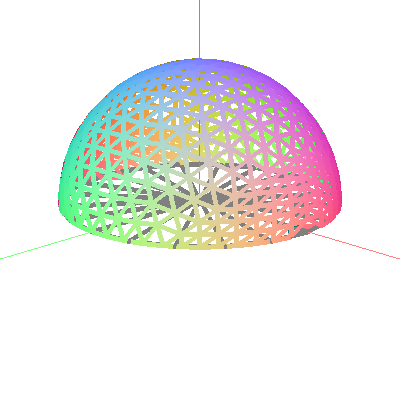
\includegraphics[width=5cm]{Figures/halficosphere3.png} }}%
  \caption{Postup generování hemisféry}%
  \label{fig:hemisfera}%
\end{figure} 

\printbibliography[title={Literatura}, heading=bibintoc]
\appendix
\end{document}